\chapter{Background}
%In the background chapter you should provide all the information required to acquire a sufficient knowledge to understand other chapters of the report. Suppose the reader is not familiar with the topic; so, for instance, if your project was focused on implementing a VPN, explain what it is and how it works. This chapter is supposed to work kind of like a "State of the Art" chapter of a thesis.\\ Organize the chapter in multiple sections and subsections depending on how much background information you want to include. It does not make any sense to mix background information about several topics, so you can split the topics in multple sections.\\Assume that the reader does not know anything about the topics and the tecnologies, so include in this chapter all the relevant information. Despite this, we are not asking you to write 20 pages in this chapter. Half a page, a page, or 2 pages (if you have a lot of information) for each `topic`(i.e. FreeRTOS, the SEcube, VPNs, Cryptomator, PUFs, Threat Monitoring....thinking about some of the projects...).%

\section{State of the art of embedded systems security approach}

The current best practice for providing a secure memory or authentication source in mobile systems is to place a secret key in nonvolatile electrically erasable programmable read-only memory (EEPROM) or battery-backed static random-access memory (SRAM) and use hardware cryptographic operations such as digital signature or encryption. Nonetheless, this approach is expensive both in terms of design and of power consumption. In addition, invasive attack mechanisms make such nonvolatile memory vulnerable. Protection against such attacks is therefore needed and it requires the use of active tamper detection/prevention circuitry which must be continually powered \cite{PUF_IEEE_Herder}.

\section{Physical unclonable functions}\label{section:physicalUnclonableFunctions}

Physical unclonable functions (PUFs) are innovative primitives that derive secrets from complex physical characteristics of the ICs rather that storing the secret in digital memory. Because the PUF taps into the random variation during an IC fabrication process, the secret is extremely difficult to predict or extract. PUFs generate volatile secrets that only exist in a digital form when a chip is powered on and running. This requires the adversary to mount the attack while the IC is running and using the secret, which is significantly harder that discovering non-volatile keys. An invasive attack must measure the PUF delays without altering them or triggering sensing wires that clear out the registers \cite{PUF_Suh_Devadas}.

The concept of PUFs is based on the idea that even though the mask and manufacturing process is the same during the creation of the same type of IC, each IC is actually slightly different due to normal manufacturing variability. PUFs leverage this variability to derive the silicon "biometric", a "secret" information that is unique to the chip. This implies that no two identical chips can be manufactured.  
Although the use of PUFs is a relatively new technology, it should be noted that the concepts of unclonability and uniqueness of objects have been extensively used in the past \cite{PUF_IEEE_Herder}.

\subsection{Types of PUFs}
Most of the currently used PUFs fall into two categories: 
\begin{itemize}
\item strong PUFs, mainly used for authentication, and 
\item weak PUFs, primarily used for key storage.
\end{itemize}

A PUF can be modeled as a black-box challenge-response system: an input challenge \emph{c} is passed to a PUF which returns a response \emph{r = f(c)}, where \emph{f(·)} describes the input/output relations of the PUF. The black-box model is appropriate to describe PUFs since input parameters of \emph{f(·)} are hidden from the user since they represent the innate manufacturing variability that PUFs use to generate unique challenge-response sets.

The fundamental difference between weak and strong PUFs is the domain of \emph{f(·)}, i.e., the number of unique challenges \emph{c} that the PUF can process. Weak PUFs can only support a small number of challenges (in some cases just a single challenge). On the contrary, a strong PUF can support a large enough number of challenges such that trying to determine/measure all challenge/response pairs (CRPs) within a limited timeframe is unfeasible.

Both weak and strong PUFs rely on analog physical properties of the fabricated circuit to derive secret information and therefore have noise and variability associated with them. For this reason, modern PUFs designs employ multiple error-correction techniques to mitigate the noise and improve reliability.

Examples of strong PUFs include optical and arbiter PUFs, while ring-oscillator and SRAM PUFs are example of weak ones. \cite{PUF_IEEE_Herder}

\subsection{SRAM PUF}
SRAM PUFs exploit the positive feedback loop in a SRAM. A SRAM has two stable states (used to store a 1 or a 0), and positive feedback to force the cell into one of these two state and to prevent an accidental state transition. 

Figure \ref{fig:SRAM_cell} shows a common six-transistor configuration of an SRAM consisting of cross-coupled CMOS inverters (M\textsubscript{1}-M\textsubscript{4}) and access transistors (M\textsubscript{5}-M\textsubscript{6}).

Theoretically, when a device with a SRAM is powered on and no write operation is performed, the SRAM cell exists in a metastable state where the feedback pushing the cell toward the "1" state equals the feedback pushing the cell toward the "0" state, thereby keeping the cell indefinitely in this metastable state. However, in actual implementations one feedback loop is always slightly stronger than the other due to small transistor threshold mismatches resulting from process variation. This means that the cell at start up relaxes into either the "1" or "0" state. The final state of the cell depends on the difference between two feedback loops and it is therefore not strongly impacted by temperature or power supply fluctuations. Nonetheless, if the two feedback loops are sufficiently close then random noise or other small environmental fluctuations can result in an output bit flip. Therefore, error correction of this output will be necessary. Error correction can be performed by using repeated measurement: since the relative strengths between the two feedback is relatively static, by measuring the outputs of the cell repeatedly one can assess the stability of a SRAM PUF bit and selectively use the most stable bits as the PUF output. \cite{PUF_IEEE_Herder}

\begin{figure}[h!]
\vspace{0.5cm}
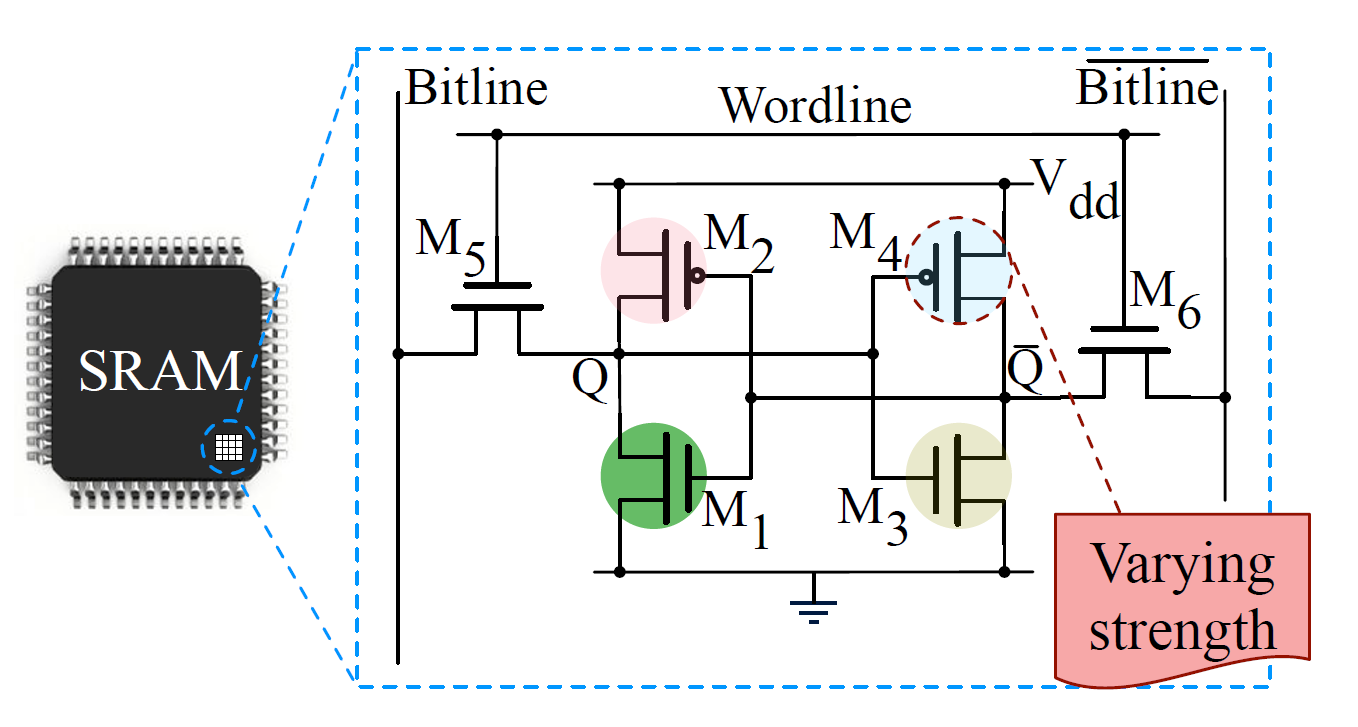
\includegraphics[width=\textwidth]{images/SRAM_cell.png}
\caption{SRAM bit cells \cite{PUF_Sutar}. }
\label{fig:SRAM_cell} % This is the image label, with which you can refer to the image in any document location.
\end{figure}


\section{SEcube\textsuperscript{TM}}
The SEcube\textsuperscript{TM} (Secure Environment cube) Open Security Platform is an open source security-oriented hardware and software platform. It provides hardware and software holistic security focusing on common operational security concepts like groups and policies instead of classical security concepts such as cryptographic algorithms and keys \cite{SEcubeDoc}. The SEcube\textsuperscript{TM} is the smallest reconfigurable silicon that combines three main cores in a single-chip design. It embeds a low-power ARM Cortex-M4 processor, a flexible and fast Field-Programmable-Gate-Array (FPGA), and an EAL5+ certified Security Controller (SmartCard), as shown in Figure \ref{fig:SEcubeComponents}. This make the SEcube\textsuperscript{TM} a secure environment since it is based on a modular software architecture where all functions are isolated \cite{SEcubeSite}.

\begin{figure}[h!]
\vspace{0.5cm}
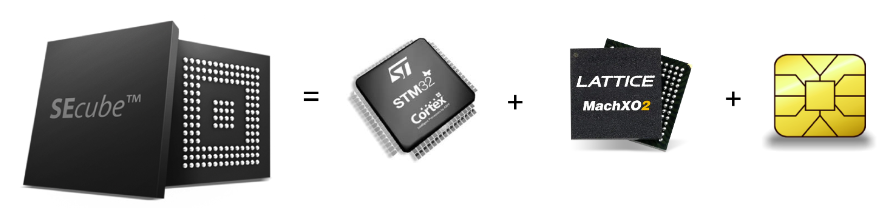
\includegraphics[width=\textwidth]{images/SEcubeComponents.png}
\caption{The three components of the SEcube\textsuperscript{TM}: the ARM Cortex-M4 processor, the FPGA and the EAL5+ SmartCard\cite{SEcubeDoc}. }
\label{fig:SEcubeComponents} % This is the image label, with which you can refer to the image in any document location.
\end{figure}





